\chapter{Network}
The Network on the Baseboard is realized through a SMSC LAN8720.\\
4-bit data nibbles are sent to the MII block. These data nibbles are clocked
to the controller at a rate of 25MHz. The controller samples the data on the
rising edge of RXCLK. To ensure that the setup and hold requirements are met,
the nibbles are clocked out of the transceiver on the falling edge of RXCLK.
RXCLK is the 25MHz output clock for the MII bus. It is recovered from the received
data to clock the RXD bus. If there is no received signal, it is derived from
system reference clock(XTAL1/CLKIN).\\
When tracking the received data, RXCLK has a miximum jitter of 0.8ns (provided
that the jitter of the input clock, XTAL1/CLKIN, is below 100ps).\\
In RMII mode, the 2-bit data nibbles are sent to the RMII block. These data nibbles
are clocked to the controller at a rate of 50MHz. The controller samples the data
on the rising edge of XTAL1/CLKIN (REF\_CLK). To ensure that the setup and hold
requirements are met, the nibbles are clocked out of the transceiver on the falling
edge of XTAL1/CLKIN (REF\_CLK).\\


The blockdiagram \ref{stm32f4_phy} shows the hardware for the RMII for
 a network connection.
\begin{figure}[ht]
	\centering
	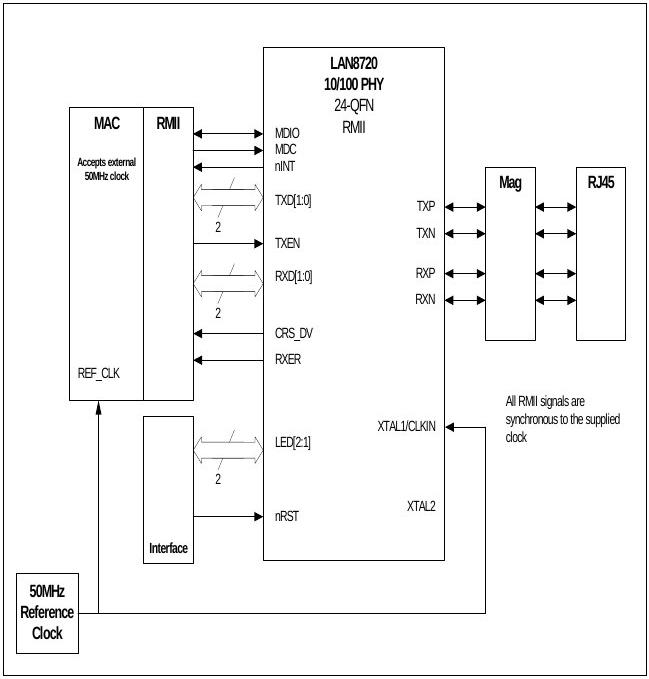
\includegraphics[width=400px,height=300px]{../img/network.jpeg}
	\caption{Blockdiagram for PHY Connection}
	\label{stm32f4_phy}
\end{figure}

